\documentclass{article}
\usepackage[utf8]{inputenc}
\usepackage{graphicx}
\usepackage[margin=1in]{geometry}
\usepackage{indentfirst}
\usepackage{hyperref}
\hypersetup{
    colorlinks=true,
    linkcolor=blue,
    filecolor=magenta,      
    urlcolor=cyan,
}
% gives version of GUI to make further editions of this document easier to make
\newcommand{\version}{v.0.1}
\newcommand{\code}[1]{\texttt{#1}}

\title{ITC-QEMU-GUI \version{} Documentation}
\author{}
\date{\today}

\begin{document}

\maketitle
\tableofcontents
\newpage


\section{Introduction}

\subsection{Purpose}
The purpose of this document is to explain the installation process, as well as the use and functionality of ITC QEMU GUI \version{}.

\subsection{Installation}
Before starting to install the GUI, make sure you have the following dependencies installed on your machine. These are all available to install from most Linux package managers.
\begin{itemize}
    \item \code{git}
    \item \code{build-essential}
    \item \code{python3}
    \item \code{python3-virtualenv}
\end{itemize}

To install the GUI, you should first create a custom build of QEMU using the provided \code{qemu\_install.sh} script. This is necessary because the GUI takes advantage of some commands which are custom and are not available in vanilla QEMU. After using the script to build QEMU, the \code{startup.sh} script is used to setup and run the GUI. Since the script must be run in the context of the current terminal, make sure to run it using \code{source startup.sh}. The script will install a python virtual environment, install necessary packages in the environment, and run the GUI. This command may be used each time you start the GUI.

To start using the GUI, you should first run an instance of QEMU, making sure to make QMP accessible. A simple example is listed below (which assumes that you have already created a bootable alpine image). If you are unsure how to get started with QEMU, refer to the itc-qemu-manual. \newline \newline
\code{\$ qemu-system-x86\_64 -qmp tcp:127.0.0.1:55555,server,nowait  ../alpine/alpine.img}
\newline

\begin{center}
    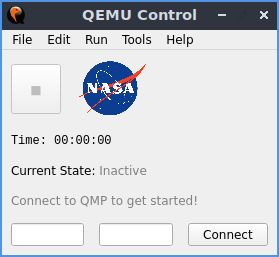
\includegraphics[]{images/main_inactive.jpg}
    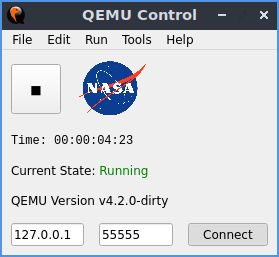
\includegraphics[]{images/main_active.jpg}
\end{center}
Once you complete the steps in the previous section you should see the main control panel of the GUI pictured above (left). If you are running QMP on port 55555 as in the example, you can just press the connect button without typing anything, and the GUI will automatically connect you to \code{localhost} on port 55555 as seen in the image on the right. Otherwise, you should type in the QMP host and port, and click the connect button. From top to bottom, you can see the pause / play button, the simulation time, the simulation state, the QEMU version, and the connect dialog. Next, we can look at some of the more advanced features that the GUI offers.

\section{Features}
The GUI offers many features that aid with debugging and using QEMU in general. The simplest feature is arguably the pause / play button on the main screen, which uses QMP to send "stop" and "continue" signals to the simulation. The following section will explore some of the more advanced features of the GUI such as the CPU Register View and the Memory dump. Keep in mind that some features of the GUI make use of not only QMP commands, but also HMP commands. To invoke HMP commands through QMP, the GUI uses the following syntax \code{\{"execute": "human-monitor-command", "arguments": \{"command-line": [HMP\_COMMAND]\}\}}
\subsection{Memory Dump}
\begin{figure}[h]
    \centering
    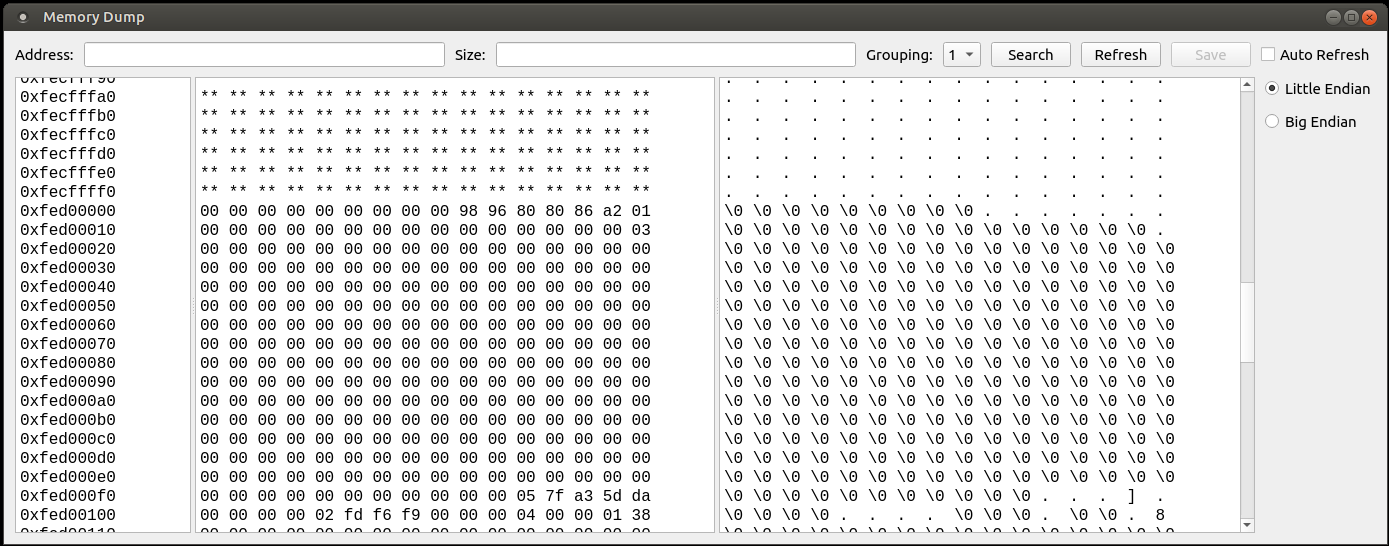
\includegraphics[width=\linewidth]{images/MemDump.PNG}
    \label{fig:memdump}
\end{figure}

The memory dump view allows users to view the contents of memory. This view displays the memory address, a hexadecimal representation of memory, and an ASCII representation of memory. To open the memory dump view, navigate to Tools $\rightarrow$ Memory Dump.

\subsubsection{Reading Memory}
To read a part of memory, specify the base address in the \textbf{Address} field. Additionally, specify the number of bytes to read in the \textbf{Size} field. If \textbf{Size} exceeds 2048, then it will be set to 2048. Finally, click \textbf{Refresh} to fetch \textbf{Size} bytes of memory starting \textbf{Address}.\par 
It is also possible to scroll up or down to load adjacent regions of memory. 

\subsubsection{Displaying Memory}\label{ReadMem}
This view automatically displays memory as bytes represented as hexadecimal and ASCII values. The \textbf{Grouping} dropdown menu can be used to set the grouping of bytes in the hexadecimal display. \textbf{Grouping} can be either 1, 2, 4, or 8, corresponding to grouping bytes, 2 btyes, 4 btyes, and 8 bytes. \par
On the right-hand side of the display, there are 2 possible selections for endianness: little endian and big endian. Selecting these displays the memory with the selected endianness. The default endianness is little endian. \par
For either of these display changes to take effect, the display must be refreshed which can be accomplished either by clicking \textbf{Refresh} or by having \textbf{Auto Refresh} selected.

\subsubsection{Auto Refresh}
The \textbf{Auto Refresh} checkbox in the top right corner controls whether the display auto refreshes or not. With \textbf{Auto Refresh} selected, the display will refresh at a rate of 10Hz. By default, \textbf{Auto Refresh} is checked.\par
\textbf{Note:} The auto refresh only refreshes the currently displayed region of memory. To load a different region the user must either scroll or follow directions as specified in \ref{ReadMem}

\subsubsection{Searching}
The \textbf{Search} button lets users search for memory at a specified address. If the address is within the currently displayed range, then the address, hexadecimal value at that address, and the ASCII value at that address will be highlighted, and the view will scroll to make them visible. If the address is not within the currently displayed range, then 1024 bytes starting at the specified address will be loaded in, and the same values will be highlighted.

\subsubsection{Saving}
The \textbf{Save} button allows the user to save the currently displayed range of memory to a file. To enable the \textbf{Save} button, the simulation must be paused.\par
\textbf{Note:} \textbf{Save} uses \code{pmemsave} to save memory to the file, so any grouping or endian display changes will not be present in the file.

\subsection{Memory Tree View}
\begin{figure}[h]
    \centering
    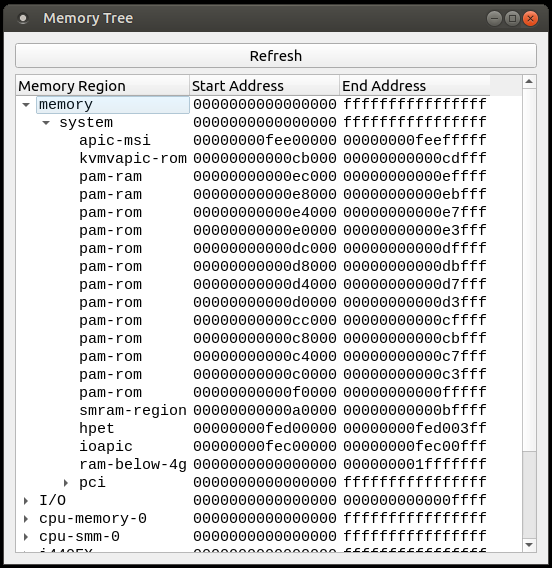
\includegraphics[width=.6\textwidth]{images/MemTree.PNG}
    \label{fig:memtree}
\end{figure}
The memory tree view displays the different regions of memory and their address ranges in the form of a tree. To open the memory tree view navigate to Tools $\rightarrow$ Memory Tree. Each region can be expanded to show its subregions. Additionally, double clicking a region opens up a memory dump view with that region displaying.
\newpage
\subsection{Assembly View}
\begin{figure}[h]
    \centering
    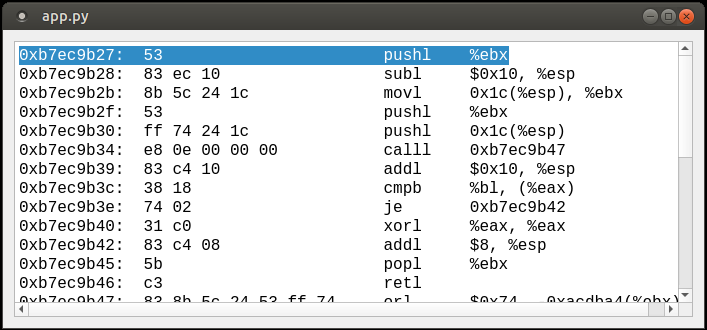
\includegraphics[width=.6\textwidth]{images/AssemblyView.PNG}
    \label{fig:asmview}
\end{figure}

The assembly view shows the current assembly instruction. To open the assembly view navigate to Tools $\rightarrow$ Assembly View. The display updates when the GUI receives a stop signal from QEMU, allowing it to work in tandem with GDB using the \code{si} or \code{ni} commands.\par
\textbf{Note:} To properly use this view, the architecture's instruction pointer register must be set in \code{package/constants.py}. By default, \code{\$eip} is used.\par
\textbf{Known Bugs:}
\begin{itemize}
    \item \code{si} and \code{ni} do not always give a stop signal when they finish stepping. Thus, sometimes the display doesn't properly update. This functionality is currently commented out.
\end{itemize}

\subsection{CPU Register View}
The CPU register view is used to view simulation CPU registers and their contents. The view can be opened by navigating to (Tools $\rightarrow$ CPU Register View). 

\begin{center}
    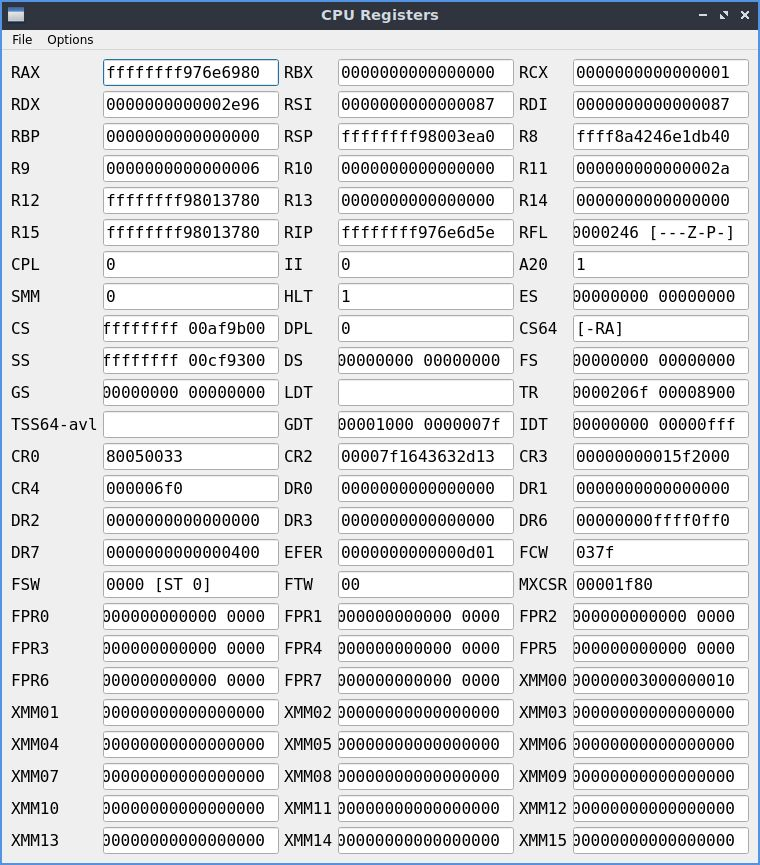
\includegraphics[width=90mm]{images/registers_fancy.jpg}
\end{center}

The register view offers options to toggle auto-refresh and to save the registers to a separate file. Finally, text mode can be toggled through the Options menu, and offers a less visually pleasing (but more organized and compact) view of the registers. \newline

\textbf{Known Limitation:}
\begin{itemize}
    \item Currently, the register view works by using the HMP command \code{info registers} to grab the text version of the CPU register values, and regex is used to parse the text. This regex is not always perfect. 
    \item In the future, a custom QMP command could be written to return a JSON object with key-value pairs, but it seems that a separate version of this command would need to be written for each separate CPU register.
\end{itemize}

\subsubsection{Searching Events}
In the top left of the trace events screen you should see a search bar. You can use this search bar to search for trace events. To the right of the search bar you should see an up arrow and a down arrow. The up arrow is used to collapse all nodes in the tree of trace events, and the down arrow is used to expand all of the nodes. 
\newpage

\subsubsection{Viewing and Saving Output}
To the right of the trace event listing you should see the past one hundred trace events. This output is saved in a file located at \code{/tmp/errors.log} and regex is used to filter out normal logging output (leaving only trace events). 
To save the output that you can see on the right of the screen to a file, navigate to File $\rightarrow$ Save to File. To disable auto-refresh, you may navigate to Options $\rightarrow$ Auto Refresh. \newline

\textbf{Note:}
\begin{itemize}
    \item The trace event window actually supports custom trace events which makes it very useful for debugging code that you may have written to customize and add to QEMU.
\end{itemize}

\subsection{Logging View}
The logging view allows you to view, save, and filter trace event logs. To open the log navigate to Tools $\rightarrow$ Logging. Whenever you select a logging option, output is stored to a logfile located at the default logging location (\code{qemu.log} in the user's home directory) or at the path specified in file prompt. The view can be seen below.
\begin{center}
    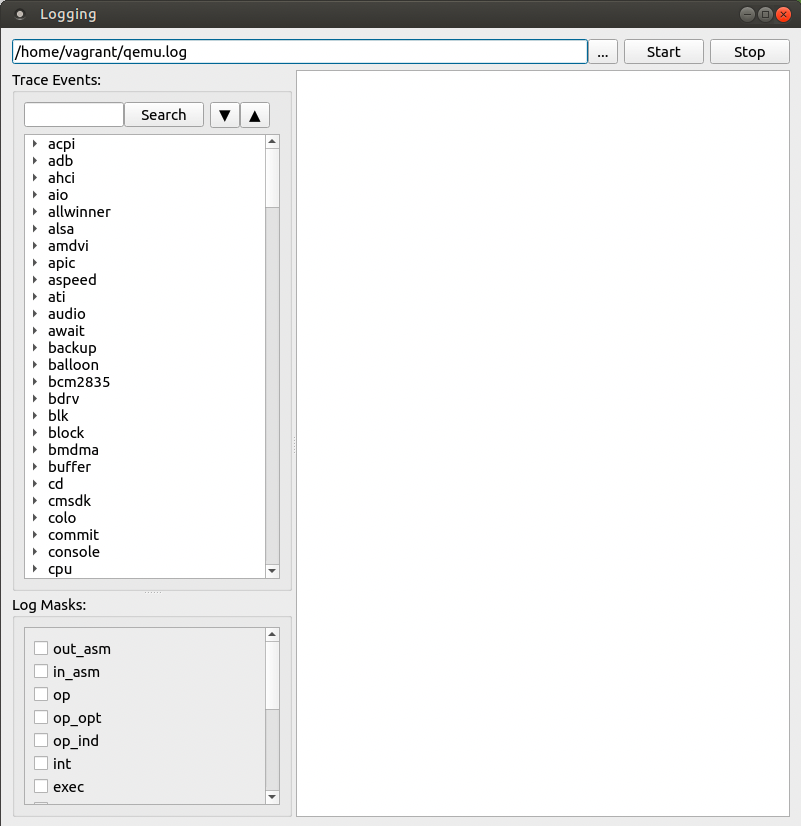
\includegraphics[width=100mm]{images/logging-view.png}
\end{center}
By default, the display will auto-refresh. There are two ways to select events to log: (1) by selecting a specific trace event (in the left dropdown view) or (2) by selecting a log mask (under the trace event dropdown view). The text entry box with the \textbf{Search} button can be used to search through the trace events dropdown view. The \textbf{Start} and \textbf{Stop} buttons can be used to start and stop logging. When logging is started, the log view is also displayed as shown below.
\begin{center}
    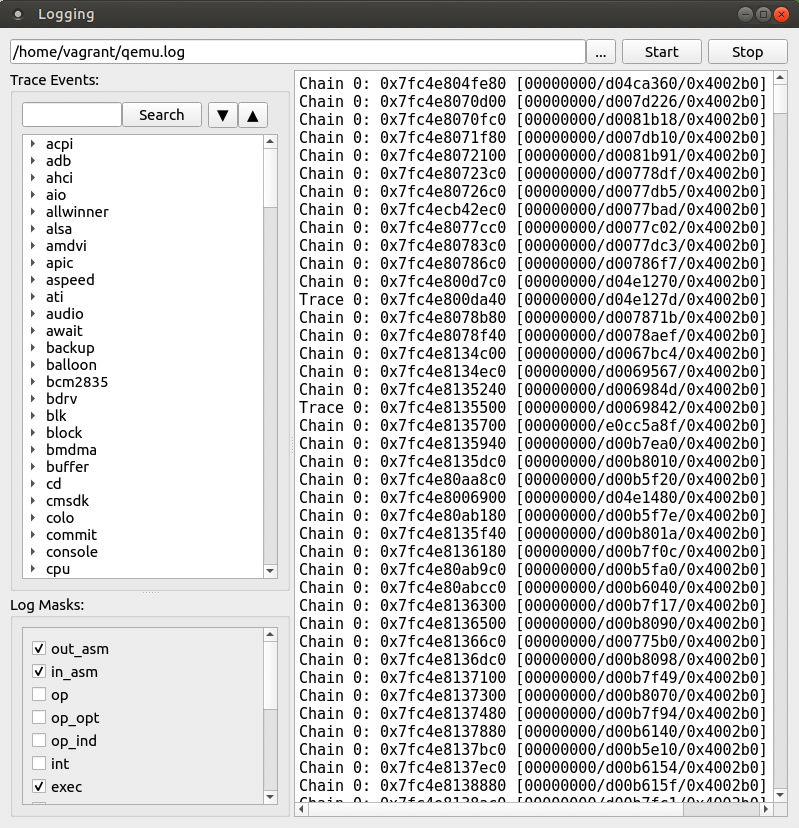
\includegraphics[width=100mm]{images/logging-view-populated.png}
\end{center}
\subsection{Time Multiplier Graph}
\begin{figure}[h]
    \centering
    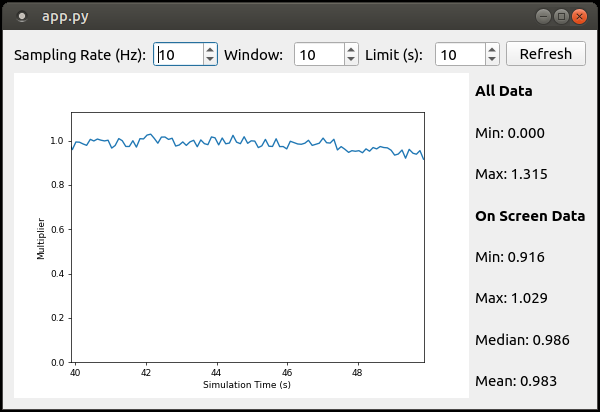
\includegraphics[width=.6\textwidth]{images/TimeMult.PNG}
    \label{fig:timemult}
\end{figure}
The time multiplier graphs real time vs. $\frac{\Delta t_{sim}}{\Delta t_{real}}$ where $t_{sim}$ is the simulation's virtual time, and $t_{real}$ is the real time. To open the time multiplier graph navigate to Tools $\rightarrow$ Time Multiplier.\par
At the top of the display, there are 3 values to alter the graph: \textbf{Sampling Rate}, \textbf{Window}, and \textbf{Limit}. \textbf{Sampling Rate}, as its name suggests, is the rate at which the simulation's time is sampled. \textbf{Window} is the number of samples used for the moving average. So, a smaller value for \textbf{Window} makes the graph change quicker, while a larger value makes the graph change slower. \textbf{Limit} is the number of seconds to display. After changing any of these values, click \textbf{Refresh} to make the changes take effect. The default value for all 3 of these values is 10.\par
On the right-hand side there are various data about the graph, including the absolute minimum, absolute maximum, and the minimum, maximum, mean, and median for values currently displayed.
\subsection{Miscellaneous}
\subsubsection{Dark Mode}
Dark mode can be enabled through the preferences dialog which contains the checkbox used to toggle dark mode (Edit $\rightarrow$ Preferences).
\begin{center}
    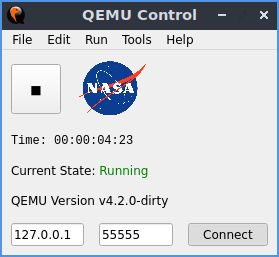
\includegraphics[]{images/main_active.jpg}
    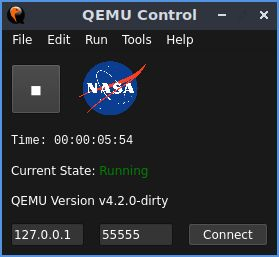
\includegraphics[]{images/main_active_dark.jpg}
\end{center}
\subsubsection{Plugin Support}
This system uses \href{https://yapsy.readthedocs.io/en/latest/}{Yapsy} as a plugin manager. To add a plugin after implementing it, specify the plugin path in \code{addPlugins} in \code{package/mainwindow.py}. Then also specify how the plugin should be handled.\par
All plugins should be accessible through the Plugins dropdown menu, which can be found by doing Tools $\rightarrow$ Plugins. Right now, the only plugin is the QMP Display which shows responses to QMP commands, as shown below.

\begin{center}
    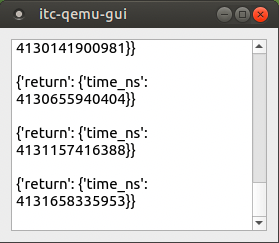
\includegraphics[width=80mm]{images/qmp-monitor-view.png}
\end{center}

\section{Added QMP Commands}

\subsection{\code{get-pmem}} \label{GetPmem}
The \code{get-pmem} command requests the contents of a part of physical memory.
\paragraph{Arguments}
\begin{itemize}
    \item \code{addr: int64}
        \subitem The starting address of the requested part of memory.
    \item \code{size: int64} 
        \subitem The number of bytes of memory being requested.
    \item \code{hash: int64} 
        \subitem A unique identifier.
    \item \code{grouping: int} 
        \subitem Specifies how many bytes each value in the return should be. Valid values are 1, 2, 4, and 8. The default value is 1.
\end{itemize}   
        
\paragraph{Return}
    \code{get-pmem} returns a \code{MemReturn} object
    \subparagraph{\code{MemReturn}}
    \begin{itemize}
        \item \code{hash: int64}
            \subitem The unique identifier passed to \code{get-pmem}.
        \item \code{vals: MemVal[]}
            \subitem An array of \code{MemVal} objects
    \end{itemize}
    
    \subparagraph{\code{MemVal}}
    \begin{itemize}
        \item \code{val: uint64}
            \subitem Single value of memory. The number of bytes \code{val} represents depends on the value of \code{grouping}.
        \item \code{ismapped: bool}
            \subitem Indicates whether that value is from a mapped region of memory or not.
    \end{itemize}
\textbf{Example:} \\
\code{-> \{"execute:" "get-pmem",} \\
\code{        "arguments": \{}\\
\code{            "addr": 4275044352,}\\
\code{"size": 1024,}\\
\code{      "hash": 0,}\\
\code{"grouping": 1 \} \}}   \\
\code{<- \{"return:" \{"hash": 0, "vals": \{"val": 0, "ismapped": true\}, \{"val": 0, "ismapped": true\}, ... \} \}}

\subsection{\code{mtree}}
The \code{mtree} command returns a tree representation of memory regions. 

\paragraph{Arguments} \code{mtree} takes no arguments.

\paragraph{Return} \code{mtree} returns an array of \code{MemoryMapEntry} objects. This array is a depth-first traversal of the tree.
\subparagraph{\code{MemoryMapEntry}}
\begin{itemize}
    \item \code{name: str}
        \subitem The name of the region of memory.
    \item \code{start: int}
        \subitem The start address of the region of memory.
    \item \code{end: int}
        \subitem The end address of the region of memory.
    \item \code{parent: str}
        \subitem The name of the parent region. A value of \code{""} indicates it is a root node. There can be multiple roots.
\end{itemize}

\textbf{Example:}\\
\code{-> \{"execute": "mtree"\}} \\
\code{<- \{"return": \{ \{"name": "memory", "start": 0, "end": -1, "parent": ""\}, \{"name": "system", "start": 0, "end": -1, "parent": "memory"\}, ... \} \}}

\subsection{\code{itc-sim-time}}
The \code{itc-sim-time} command returns the time in nanoseconds given a specified \code{ClockType}. \code{ClockType} is an enum with possible values \code{realtime, virtual, host, and virtual-rt} which all correspond to QEMU's clock type enum in \code{include/qemu/timer.h}.

\paragraph{Arguments}
\begin{itemize}
    \item \code{clock: ClockType}
        \subitem The clock type to use to get the time.
\end{itemize}

\paragraph{Return} \code{itc-sim-time} returns a \code{SimTime} object.
\subparagraph{\code{SimTime}}
\begin{itemize}
    \item \code{time\_ns: int64}
    \subitem The time in nanoseconds.
\end{itemize}

\textbf{Example:}\\
\code{->\{"execute": "itc-sim-time",}\\
\code{"arguments": \{"clock": "virtual"\} \}}\\
\code{<-\{"return": \{"time\_ns": 1040040609 \} \}}

\subsection{\code{itc-time-metric}}
The \code{itc-time-metric} command gives an array containing the current host time and the current virtual time.

\paragraph{Arguments} \code{itc-time-metric} does not take any arguments.

\paragraph{Return} \code{itc-time-metric} returns an array containing 2 \code{SimTime} objects. The first value is the virtual time, and the second value is the host time.

\textbf{Example:}\\
\code{->\{"execute": "itc-time-metric" \}}\\
\code{<-\{"return": \{ \{"time\_ns": 1040040609\}, \{"time\_ns": 1594065163483704\} \} \}}
\end{document}
